\section{Observations}

Refer Fig. \ref{circuit},
\begin{itemize}
    \item $R_1 = 2.152$ \kohm
    \item $R = 0.988$ \kohm, $R' = 0.987$ \kohm, $R'' = 0.995$ \kohm
    \item $C = 97.8$ nF, $C' = 93.2$ nF, $C'' = 98.6$ nF
\end{itemize}

$\therefore$ average value of $R=0.990$ \kohm, $C=96.53$ nF\\
$\implies$ From Eqn. (\ref{freq}), theoretical value of oscillating frequency = 679.88 Hz.\\

\textbf{Observed Values:}

\begin{itemize}
    \item $R_f$ at oscillating frequency = 80.6 \kohm
    \item Minimum gain required to sustain oscillations = $|R_f/R_1| = 37.45$
    \item Experimental value of Oscillating frequency = 719.4 Hz
    \item Oscillating frequency obtained from the Lissajous figure = 720 Hz
\end{itemize}

\begin{figure}[H]
    \centering
    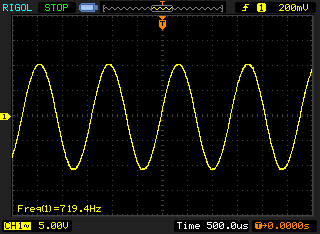
\includegraphics[width=0.8\columnwidth]{images/resonant.png}
    \caption{Sinusoidal waveform obtained at $R_f=80.6$ \kohm\,and oscillating frequency = 719.4 Hz}
    \label{res}
\end{figure}

The variable resistor ($R_f$) value was increased until the sinusoidal waveform was obtained on the oscilloscope (Fig. \ref{res}). Furthermore, using a function generator a secondary signal was fed into the oscilloscope in X-Y mode and various kinds of Lissajous curves were obtained (Fig. \ref{l1} to \ref{l4}).

\begin{figure}[H]
    \centering
    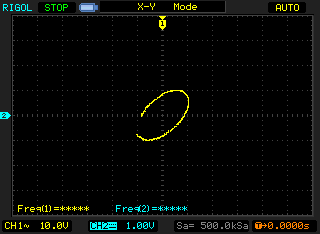
\includegraphics[width=0.8\columnwidth]{images/lissajous1.png}
    \caption{Elliptical Lissajous figure obtained when the frequency of the function generator matched the oscillating frequency of the circuit ($\approx 720$ Hz)}
    \label{l1}
\end{figure}

\begin{figure}[H]
    \centering
    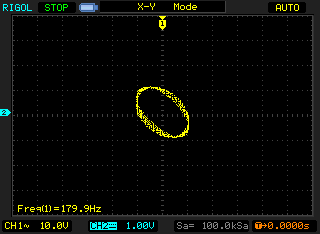
\includegraphics[width=0.75\columnwidth]{images/lissajous2.png}
    \caption{Lissajous figure obtained at a frequency lower than the resonant frequency}
    \label{l2}
\end{figure}

\begin{figure}[H]
    \centering
    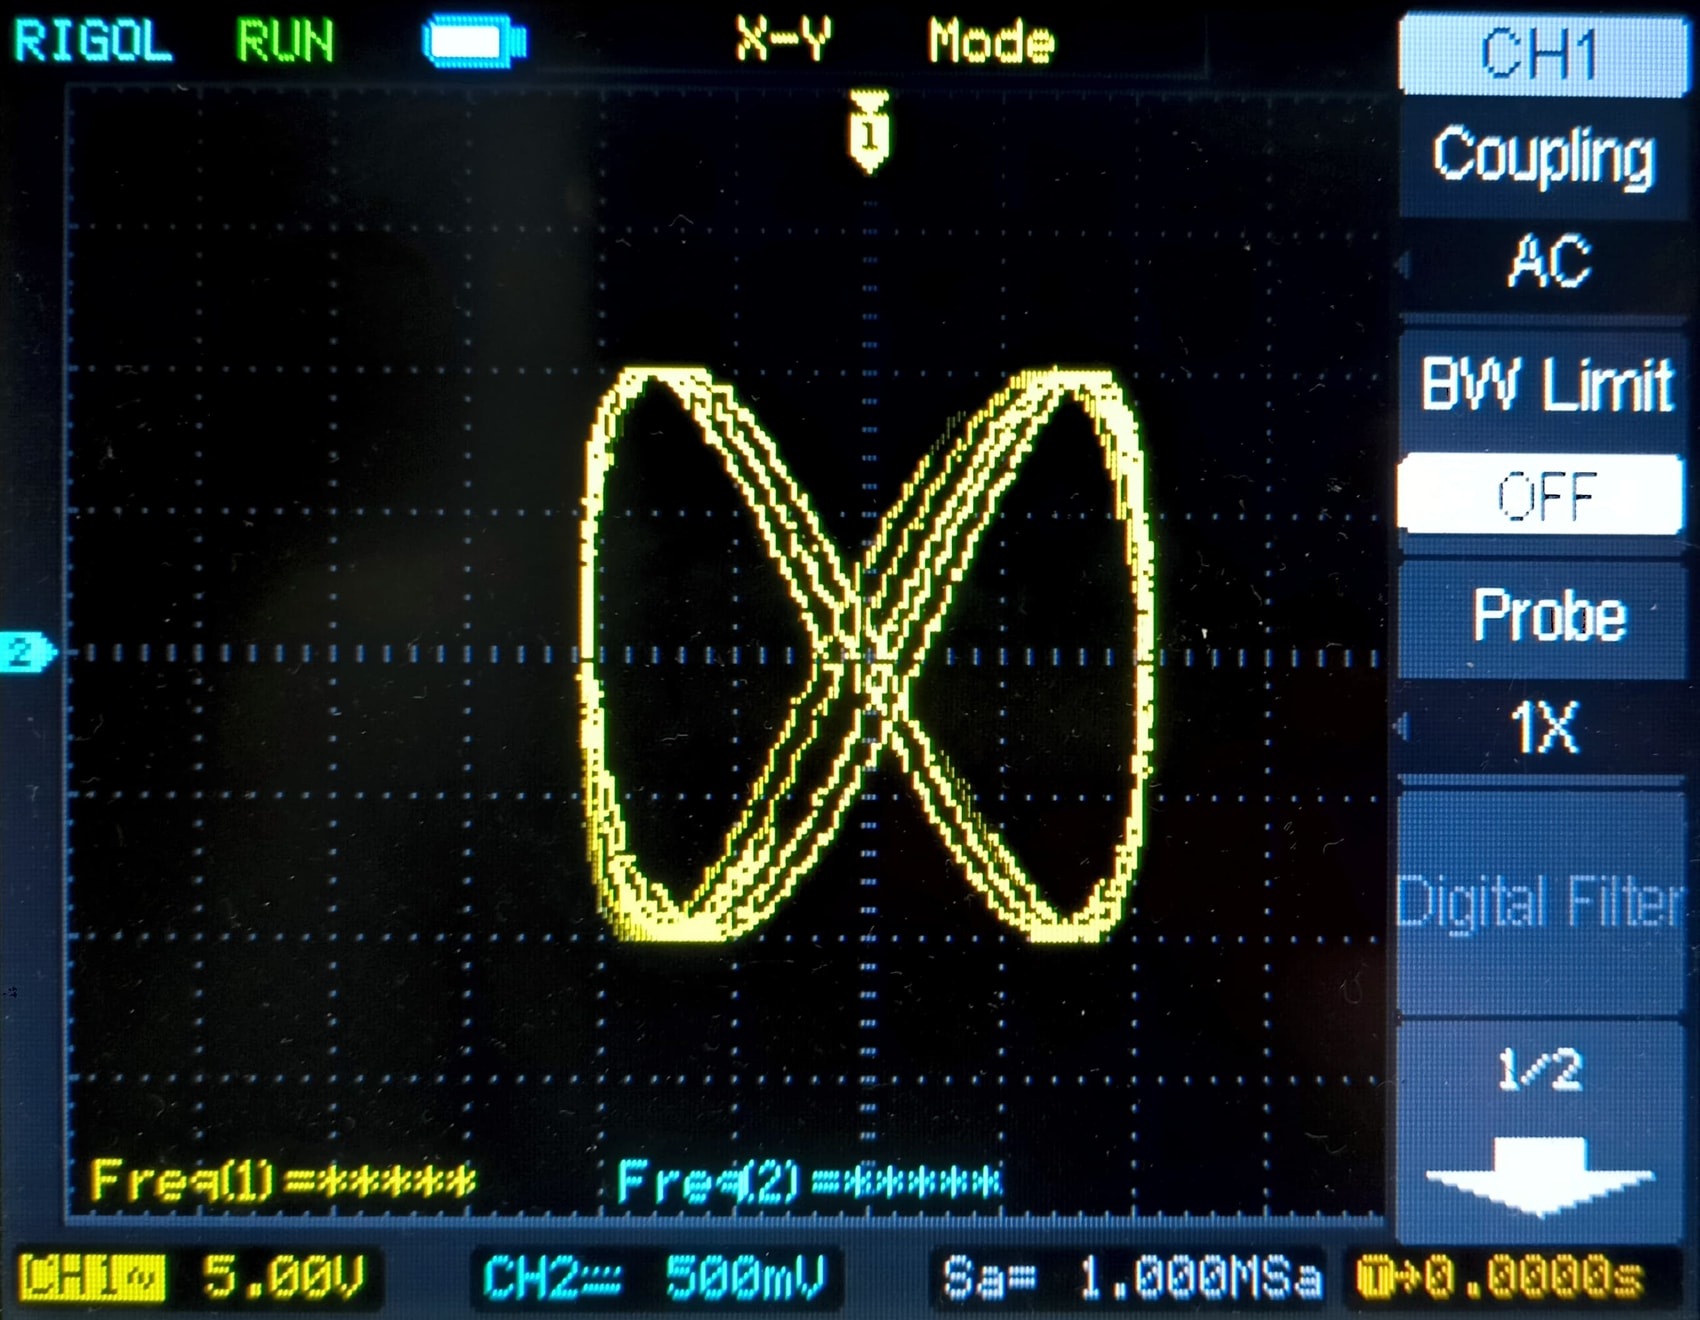
\includegraphics[width=0.75\columnwidth]{images/l3.jpg}
    \caption{Lissajous figure obtained at a frequency close to the second harmonic of the resonant frequency ($\approx 1.5$ kHz)}
    \label{l3}
\end{figure}

\begin{figure}[H]
    \centering
    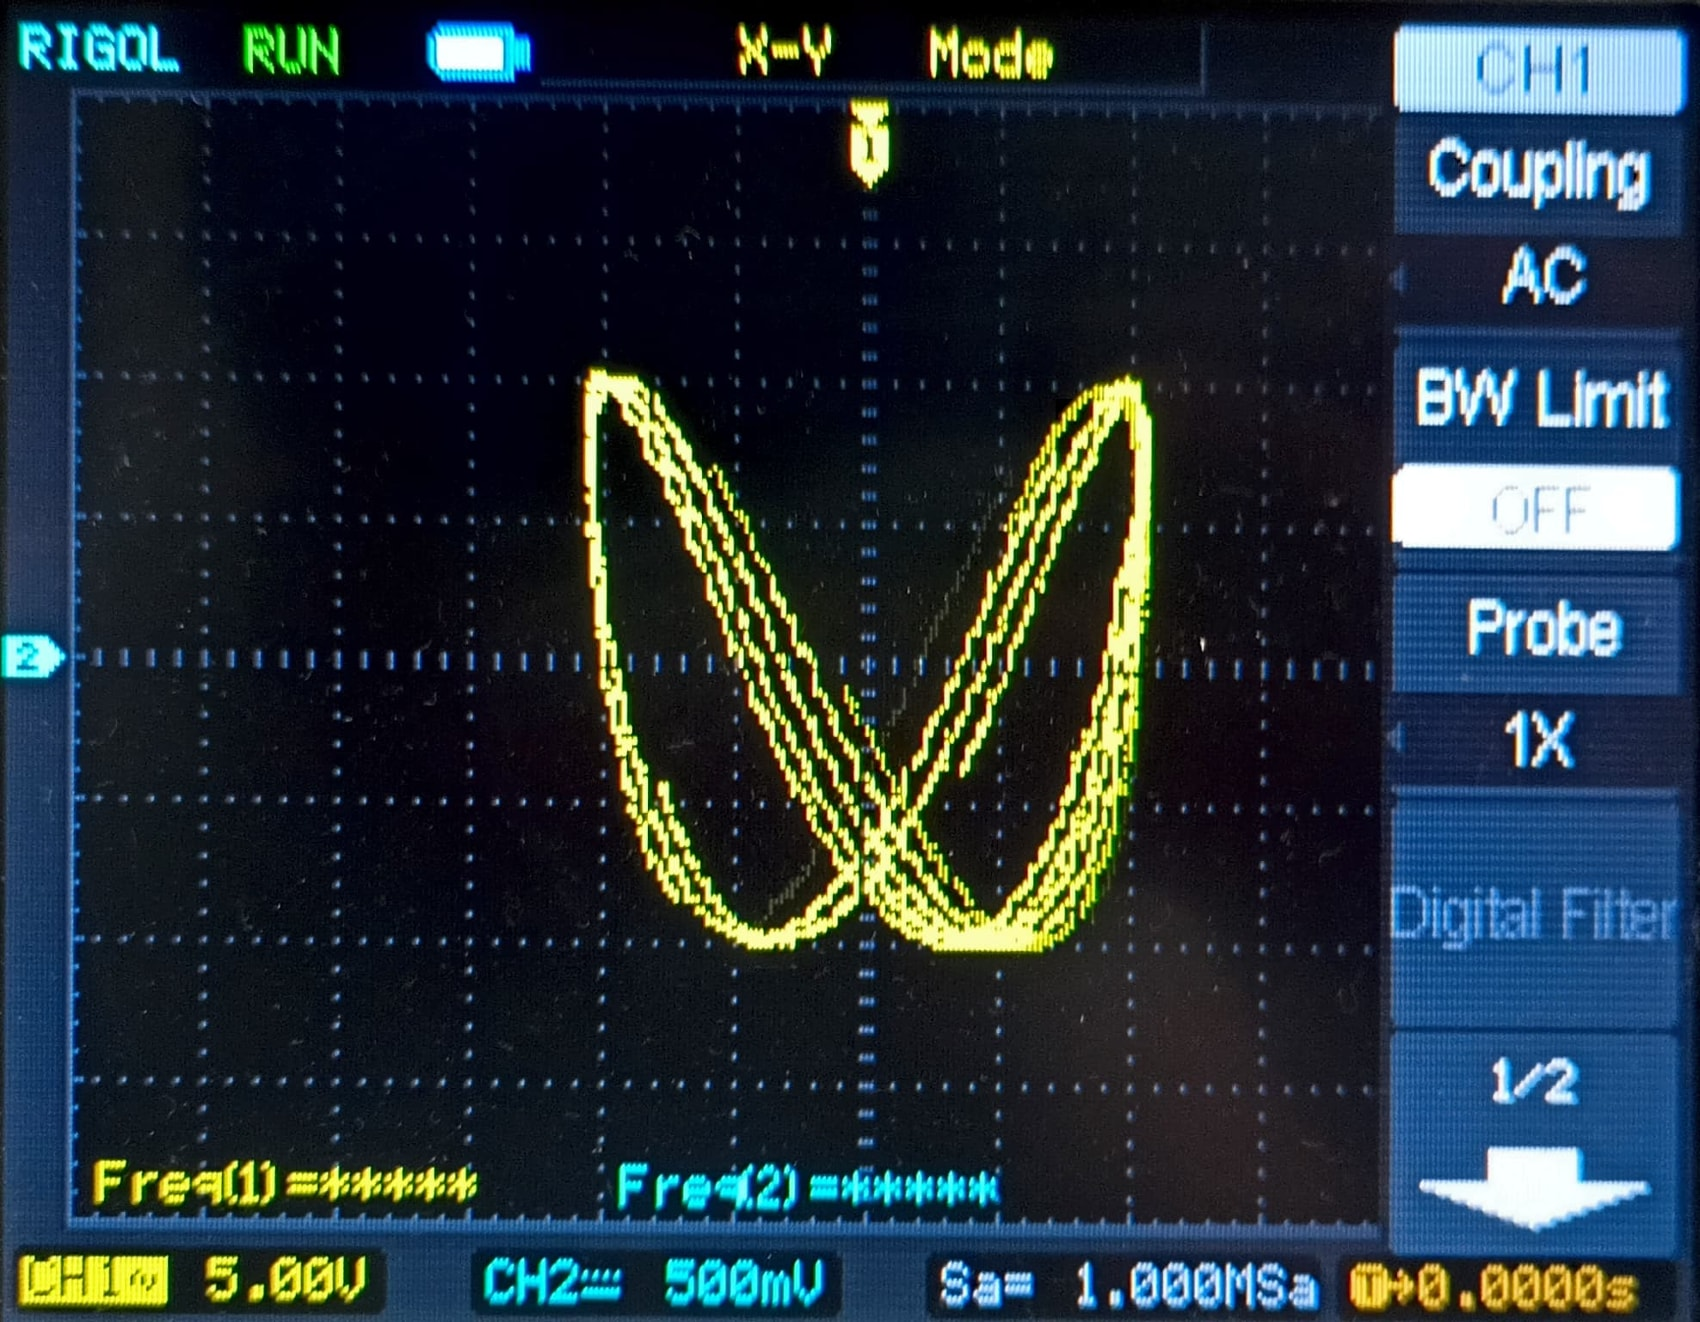
\includegraphics[width=0.75\columnwidth]{images/l4.jpg}
    \caption{Lissajous figure obtained at a higher frequency}
    \label{l4}
\end{figure}